\de{ĐỀ THI HỌC KỲ I NĂM HỌC 2022-2023}{THPT Trường Chinh - Đề số 3}



% Câu 1
\begin{bt}%[0T1B3-5]%[Dự án đề kiểm tra HKI NH22-23 - Quan Ón]%[Trường Chinh - Đề 3]
	Cho $A=(-2; 4)$ và $B=(-\infty; 3]$. Tìm $A \cap B$, $A\cup B$, $A \setminus B$, $B \setminus A$.\\
	\dapso{$A \cap B=(-2;3]$; $A\cup B=(-\infty;4)$; $A \setminus B=(3;4)$; $B \setminus A=(-\infty;-2]$.}
	\loigiai{
	Vì $A=(-2; 4)$ và $B=(-\infty; 3]$ nên ta có
	\begin{itemize}
		\item $A \cap B=(-2;3]$.
		\item $A\cup B=(-\infty;4)$.
		\item $A \setminus B=(3;4)$.
		\item $B \setminus A=(-\infty;-2]$.
	\end{itemize}
}
\end{bt}

% Câu 2
\begin{bt}%[0T2B2-3]%[Dự án đề kiểm tra HKI NH22-23 - Quan Ón]%[Trường Chinh - Đề 3]
	Biểu diễn miền nghiệm của hệ bất phương trình: $\heva{&x-2 y+4 \geq 0\\&3 x+y-6 \leq 0.}$\\
	\dapso{
		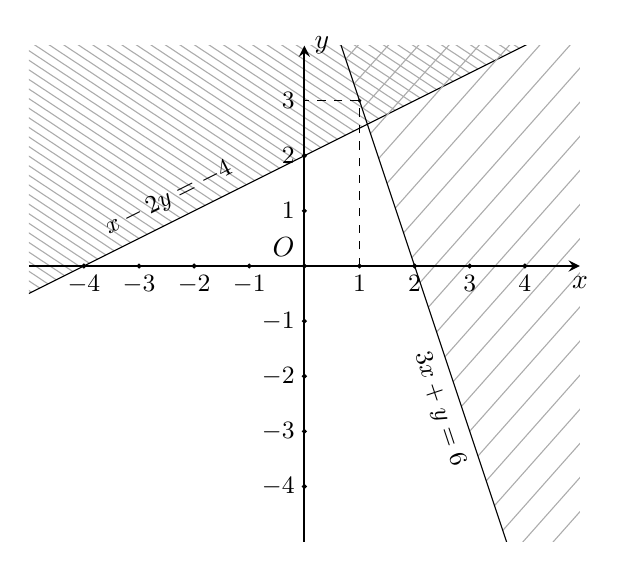
\begin{tikzpicture}[>=stealth,smooth,samples=100,scale=.7]
			\begin{scope}
				\clip (-5,-5) rectangle (5,4);
				%% Hàm thứ 1-----------------
				\pgfmathsetmacro{\goc}{-atan(-0.5)+120}
				\foreach \i in {-12,-11.85,...,11}{
					\draw[gray!65,thin]({\i},{(-1*\i-4)/-2})--+(\goc:15);}
				\draw plot[domain=-10:10]({\x},{(-1*\x-4)/-2});
				\path (-1,1.5)--(1,2.5) node[sloped,pos=-.55,shift={({\goc+150}:-9pt)},font=\small]{$x-2y = -4$};
				%% Hàm thứ 2-----------------
				\pgfmathsetmacro{\goc}{-atan(3)+120}
				\foreach \i in {-12,-11.85,...,11}{
					\draw[gray!65,thin]({\i},{(-3*\i--6)/1})--+(\goc:15);}
				\draw plot[domain=-10:10]({\x},{(-3*\x--6)/1});
				\path (-1,9)--(1,3) node[sloped,pos=2.1,shift={({\goc+150}:25pt)},font=\small]{$3x + y = 6$};
			\end{scope}
		    \fill (1,3) circle (1pt);
			\draw[->,thick] (-5,0)--(5,0)node[below]{$x$};
			\draw[->,thick] (0,-5)--(0,4)node[right]{$y$};
			\draw[fill=black] (0,0) circle (1pt) node[above left]{$O$};
			\foreach \x in {
				-4,-3,-2,-1,1,2,3,4
			}{
				\draw[fill=black] (\x,0)node[below]{\small $\x$} circle (1pt);
			}
			\foreach \y in {
				-4,-3,-2,-1,1,2
			}{
				\draw[fill=black] (0,\y)node[left]{\small $\y$} circle (1pt);
			}
			\draw[dashed] (1,0)--(1,3)--(0,3)node[left]{\small $3$};
		\end{tikzpicture}	
	}
    \loigiai{
    - Vẽ hai đường thẳng $x - 2y = -4$ và $3x + y = 6$.\\
    - Biểu diễn miền nghiệm của từng bất phương trình trong hệ trên cùng một mặt phẳng tọa độ.\\
    - Miền nghiệm $D$ của hệ bất phương trình đã cho là miền không được tô (kể cả các đường biên).
    \begin{center}
    	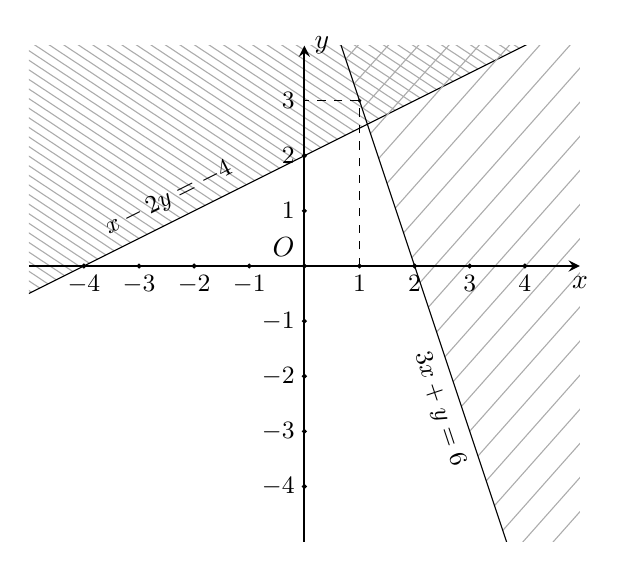
\begin{tikzpicture}[>=stealth,smooth,samples=100,scale=.7]
    		\begin{scope}
    			\clip (-5,-5) rectangle (5,4);
    			%% Hàm thứ 1-----------------
    			\pgfmathsetmacro{\goc}{-atan(-0.5)+120}
    			\foreach \i in {-12,-11.85,...,11}{
    				\draw[gray!65,thin]({\i},{(-1*\i-4)/-2})--+(\goc:15);}
    			\draw plot[domain=-10:10]({\x},{(-1*\x-4)/-2});
    			\path (-1,1.5)--(1,2.5) node[sloped,pos=-.55,shift={({\goc+150}:-9pt)},font=\small]{$x-2y = -4$};
    			%% Hàm thứ 2-----------------
    			\pgfmathsetmacro{\goc}{-atan(3)+120}
    			\foreach \i in {-12,-11.85,...,11}{
    				\draw[gray!65,thin]({\i},{(-3*\i--6)/1})--+(\goc:15);}
    			\draw plot[domain=-10:10]({\x},{(-3*\x--6)/1});
    			\path (-1,9)--(1,3) node[sloped,pos=2.1,shift={({\goc+150}:25pt)},font=\small]{$3x + y = 6$};
    		\end{scope}
    		\fill (1,3) circle (1pt);
    		\draw[->,thick] (-5,0)--(5,0)node[below]{$x$};
    		\draw[->,thick] (0,-5)--(0,4)node[right]{$y$};
    		\draw[fill=black] (0,0) circle (1pt) node[above left]{$O$};
    		\foreach \x in {
    			-4,-3,-2,-1,1,2,3,4
    		}{
    			\draw[fill=black] (\x,0)node[below]{\small $\x$} circle (1pt);
    		}
    		\foreach \y in {
    			-4,-3,-2,-1,1,2
    		}{
    			\draw[fill=black] (0,\y)node[left]{\small $\y$} circle (1pt);
    		}
    		\draw[dashed] (1,0)--(1,3)--(0,3)node[left]{\small $3$};
    	\end{tikzpicture}
    \end{center}
}
\end{bt}

% Câu 3
\begin{bt}%[0T3B1-2]%[Dự án đề kiểm tra HKI NH22-23 - Quan Ón]%[Trường Chinh - Đề 3]
	Tìm tập xác định của hàm số $y=\dfrac{|x-2|-\sqrt{5+2x}}{3-2x}$. \dapso{$\mathscr{D} = \left[-\dfrac{5}{2};+\infty\right)\setminus\left\{\dfrac{3}{2}\right\}$.}
	\loigiai{
	Điều kiện xác định của hàm số đã cho là
	$$ \heva{&5 + 2x \geq 0\\& 3 - 2x \neq 0} \Leftrightarrow \heva{&x \geq - \dfrac{5}{2}\\&x \neq \dfrac{3}{2}} \Leftrightarrow x \in \left[-\dfrac{5}{2};+\infty\right)\setminus\left\{\dfrac{3}{2}\right\}. $$
	Vậy tập xác định của hàm số đã cho là $\mathscr{D} = \left[-\dfrac{5}{2};+\infty\right)\setminus\left\{\dfrac{3}{2}\right\}$.
}
\end{bt}

% Câu 4
\begin{bt}%[0T3B2-2]%[Dự án đề kiểm tra HKI NH22-23 - Quan Ón]%[Trường Chinh - Đề 3]
	Tìm các số $b$, $c$ sao cho đồ thị hàm số $y=x^2+bx+c$ là một parabol có đỉnh $I(2; 5)$.\\
	\dapso{$b=-4$; $c=9$.}
	\loigiai{
	Vì đồ thị hàm số có hoành độ đỉnh là $x_{I} = - \dfrac{b}{2a} \Leftrightarrow 2 = -\dfrac{b}{2} \Rightarrow b = -4$. $\hfill (1)$\\
	Hơn nữa, đồ thị hàm số đi qua điểm $I(2;5)$ nên ta có $5 = 2^2 + b\cdot 2 + c \Leftrightarrow 2b + c = 1$. $\hfill (2)$\\
	Từ $(1)$ và $(2)$, ta có hệ phương trình
	$$ \heva{&b = -4\\& 2b + c = 1} \Leftrightarrow \heva{&b = -4\\&c = 9.} $$
	Vậy $b = -4$; $c = 9$ và $y = x^2 - 4x + 9$.
}
\end{bt}

% Câu 5
\begin{bt}%[0T6B4-1]%[Dự án đề kiểm tra HKI NH22-23 - Quan Ón]%[Trường Chinh - Đề 3]
	Điểm kiểm tra giữa học kì 9 môn của bạn An như sau:
	$$ 7; 8; 5; 6; 8; 7; 5; 9; 8. $$
	Tìm số trung bình, trung vị, tứ phân vị, khoảng biến thiên của mẫu số liệu trên.\\
	\dapso{$\overline{x}=7$; $M_e=7$; $Q_1=5{,}5; Q_2=7; Q_3=8$; $R=4$.}
	\loigiai{
	- Điểm trung bình cộng của bạn An là
	$$ \bar{x} = \dfrac{1}{9}(7 + 8 + 5 + 6 + 8 + 7 + 5 + 9 + 8) = 7. $$
	Sắp xếp lại mẫu số liệu theo thứ tự không giảm, ta được
	$$ 5; 5; 6; 7; 7; 8; 8; 8; 9. $$
	- Khoảng biến thiên của mẫu số liệu là $R = 9 - 5 = 4$.\\
	- Cỡ mẫu là $n = 9$ là số lẻ nên giá trị phân vị thứ hai là $M_e = Q_2 = 7$.\\
	- Tứ phân vị thứ nhất là trung vị của mẫu $5; 5; 6; 7$. Do đó, $Q_1 = \dfrac{5 + 6}{2} = 5{,}5$.\\
	- Tứ phân vị thứ ba là trung vị của mẫu $8; 8; 8; 9$. Do đó, $Q_3 = \dfrac{8 + 8}{2} = 8$.
}
\end{bt}

% Câu 6
\begin{bt}%[0T4B2-1]%[Dự án đề kiểm tra HKI NH22-23 - Quan Ón]%[Trường Chinh - Đề 3]
	Cho tam giác $ABC$ có $AB=5, AC=6, BC=8$. Tính góc $A$, diện tích tam giác $ABC$, độ dài đường cao $BK$, bán kính đường tròn nội tiếp tam giác $ABC$.\\ \dapso{$\widehat{A}\approx 92^\circ 52'$; $S=\dfrac{3\sqrt{399}}{4}$; $BK=\dfrac{\sqrt{399}}{4}$; $ r=\dfrac{3\sqrt{399}}{38}$.}
	\loigiai{
	\begin{center}
		\begin{tikzpicture}[>=stealth,line join=round,line cap=round,font=\footnotesize,scale=1]
			\path
			(1.7,2) coordinate (A)
			(0,0) coordinate (B)
			(5,0) coordinate (C);
			\draw (A)--(B)--(C)--(A);
			\fill ($(A)!0.5!(B)$) node[shift={(120:3mm)}]{$5$};
			\fill ($(A)!0.5!(C)$) node[shift={(60:3mm)}]{$6$};
			\fill ($(B)!0.5!(C)$) node[shift={(-90:3mm)}]{$8$};
			\foreach \p/\r in {A/90,B/-135,C/-45}
			\fill (\p) circle (1.2pt) node[shift={(\r:3mm)}]{$\p$};
		\end{tikzpicture}
	\end{center}
	Xét tam giác $ABC$, áp dụng hệ quả của định lí cosin, ta có
	$$ \cos A = \dfrac{b^2 + c^2 - a^2}{2bc} = \dfrac{6^2 + 5^2 - 8^2}{2\cdot 6\cdot 5} = -\dfrac{1}{20} \Rightarrow \widehat{A} \approx 92^\circ52'. $$
	Vì $\widehat{A} \approx 92^\circ52'$ là góc lẻ nên ta sẽ dùng công thức Hê - rông để tính diện tích.\\
	Nửa chu vi của tam giác $ABC$ là $p = \dfrac{a + b +c}{2} = \dfrac{8 + 6 + 5}{2} = 9{,}5$.\\
	Do đó, diện tích tam giác $ABC$ là
	$$ S_{\triangle ABC} = \sqrt{p(p-a)(p-b)(p-c)} = \sqrt{9{,}5(9{,}5 - 8)(9{,}5 - 6)(9{,}5 - 5)} = \dfrac{3\sqrt{399}}{4}. $$
	Mặt khác, ta có $S_{\triangle ABC} = \dfrac{1}{2}BK\cdot AC \Rightarrow BK = \dfrac{2S_{\triangle ABC}}{AC} = \dfrac{2\cdot \dfrac{3\sqrt{399}}{4}}{6} = \dfrac{\sqrt{399}}{4}$.\\
	Ta cũng có $S_{\triangle ABC} = pr \Rightarrow r = \dfrac{S_{\triangle ABC}}{p} = \dfrac{\dfrac{3\sqrt{399}}{4}}{9{,}5} = \dfrac{3\sqrt{399}}{38}$.
}
\end{bt}

% Câu 7
\begin{bt}%[0T5B2-2]%[0T5B4-1]%[Dự án đề kiểm tra HKI NH22-23 - Quan Ón]%[Trường Chinh - Đề 3]
	\begin{listEX}
		\item Cho tứ giác $ABCD$. Chúng minh rằng: $\overrightarrow{A C}+\overrightarrow{BD}=\overrightarrow{AD}-\overrightarrow{CB}$.
		\item  Cho tam giác $ABC$ có $M$ là trung điểm cạnh $AB$. Điểm N thoả điều kiện $\overrightarrow{BC}=\dfrac{2}{5} \overrightarrow{BN}$. Tính vecto $\overrightarrow{MN}$ theo hai vecto $\overrightarrow{CA}, \overrightarrow{CB}$. \dapso{$\overrightarrow{MN}=-\dfrac{1}{2}\overrightarrow{CA}-2\overrightarrow{CB}$.}
		\item  Cho hình chữ nhât $ABCD$ có $AD=6, AB=8$. Tính tích vô hướng $\overrightarrow{AB} \cdot \overrightarrow{AC}$. \dapso{$64$.}
	\end{listEX}
    \loigiai{
    \begin{enumerate}
    	\item Ta có $\overrightarrow{AC} + \overrightarrow{BD} = \overrightarrow{AD} + \overrightarrow{DC} + \overrightarrow{BC} + \overrightarrow{CD} = \overrightarrow{AD} - \overrightarrow{CB} + \overrightarrow{DC} + \overrightarrow{CD} = \overrightarrow{AD} - \overrightarrow{CB}$.
    	\item Ta có $\begin{aligned}[t]
    		\overrightarrow{MN} &= \overrightarrow{MC} + \overrightarrow{CB} + \overrightarrow{BN}\\
    		&= -\dfrac{1}{2}\left( \overrightarrow{CA} + \overrightarrow{CB} \right) + \overrightarrow{CB} + \dfrac{5}{2}\overrightarrow{BC}\\
    		&= -\dfrac{1}{2}\overrightarrow{CA} - 2\overrightarrow{CB}.
    	\end{aligned}$\\
        Vậy $\overrightarrow{MN}=-\dfrac{1}{2}\overrightarrow{CA}-2\overrightarrow{CB}$.
        \item 
        Vì $ABCD$ là hình chữ nhật nên $BC = AD = 6$, $CD = AB = 8$.
        \immini{
        Xét tam giác $ABC$ vuông tại $B$, ta có\\
        $AC^2 = AB^2 + BC^2 = 8^2 + 6^2 = 100 \Rightarrow AC = 10$.\\
        Suy ra $\cos\widehat{BAC} = \dfrac{AB}{AC} = \dfrac{8}{10} = \dfrac{4}{5}$.\\
        Do đó, ta có
        $$ \overrightarrow{AB}\cdot\overrightarrow{AC} = \left| \overrightarrow{AB}\right|\cdot\left|\overrightarrow{AC} \right|\cdot \cos\widehat{BAC} = 8\cdot 10\cdot\dfrac{4}{5} = 64. $$
    }{
        \begin{tikzpicture}[>=stealth,line join=round,line cap=round,font=\footnotesize,scale=1]
        	\path
        	(0,3) coordinate (A)
        	(4,3) coordinate (B)
        	(4,0) coordinate (C)
        	(0,0) coordinate (D);
        	\draw (A)--(B)--(C)--(D)--(A)--(C);
        	\fill ($(A)!0.5!(B)$) node[shift={(90:3mm)}]{$8$};
        	\fill ($(A)!0.5!(D)$) node[shift={(180:3mm)}]{$6$};
        	\foreach \p/\r in {A/135,B/45,C/-45,D/-135}
        	\fill (\p) circle (1.2pt) node[shift={(\r:3mm)}]{$\p$};
        	\foreach \a/\b/\c in {A/B/C, B/C/D, C/D/A, D/A/B} {\draw pic [draw, angle radius=2mm] {right angle=\a--\b--\c};}
        \end{tikzpicture}
}
    \end{enumerate}
}
\end{bt}

% Câu 8
\begin{bt}%[0T5T4-1]%[0T4T2-1]%[0T2K2-2]%[Dự án đề kiểm tra HKI NH22-23 - Quan Ón]%[Trường Chinh - Đề 3]
	\begin{listEX}
		\item Trong Vật lí, tích vô hướng của $\overrightarrow{F}$ và $\overrightarrow{d}$ biểu diễn công $A$ sinh bởi lực $\overrightarrow{F}$ khi thực hiện độ dịch chuyển $\overrightarrow{d}$. Một người dùng một lực $\overrightarrow{F}$ có cường độ $15 \mathrm{~N}$ kéo một chiếc xe đi quãng đường dài $30 \mathrm{~m}$. Tính công sinh bởi lực $\overrightarrow{F}$, biết rằng góc giữa vecto $\overrightarrow{F}$ và hướng di chuyển là $30^{\circ}$. \dapso{$225\sqrt{3}$ J.}
		\item 
		\immini{
			Để đo khoảng cách từ vị trí $A$ đến vị trí $B$ ở hai bên bờ hồ, bạn An đi dọc bờ hồ từ vị trí $A$ đến vị trí $C$ và tiến hành đo các góc $BAC$ và $BCA$. Biết $AC=25$ m, $\widehat{BAC}=58{,}95^{\circ}$, $\widehat{BCA}=83{,}15^{\circ}$ ( tham khảo hình bên). Hỏi, khoảng cách từ vị trí $A$ đến vị trí $B$ là bao nhiêu mét? \dapso{$40{,}41$ m.}
		}{
			\begin{tikzpicture}[scale=1,font=\footnotesize,line cap=round,line join=round,>=stealth]
				\def\a{3.75}
				\path (0:0) coordinate(A) (58.95:1) coordinate(a) (0:\a) coordinate(C)  + (96.85:1) coordinate(c)  (intersection of A--a and C--c) coordinate(B);
				\fill[cyan!60] (-.5,2) .. controls +(-70:2) and +(150:1) .. (2.5,1) .. controls +(-15:2) and +(-30:1) .. (4.5,3.5) .. controls +(150:1) and +(40:1) .. (2,4) .. controls +(-150:1.5) and +(100:2) .. cycle;
				\draw (A)--(B)--(C)--cycle;
				\foreach \d/\g in {A/-135, B/90, C/-45}
				\fill (\d) circle(1pt) node[shift={(\g:.3)}]{$\d$};
				\path (A)--(C) node[midway,below]{$25$ m} pic[draw,angle radius=.3cm]{angle=C--A--B} (A) node[shift={(20:.8)}]{$58{,}95^\circ$} pic[draw,angle radius=.3cm]{angle=B--C--A} pic[draw,angle radius=.35cm]{angle=B--C--A} (C) node[shift={(150:.7)}]{$83{,}15^\circ$};			
			\end{tikzpicture}
		}
		\item Một người bán nước giải khát đang có $48$ g bột cam, 18 l nước và $420$ g đường để pha chế hai loại nước cam $A$ và $B$. Để pha chế $1$ l nước cam loại $A$ cần $30$ g đường, $1$ l nước và $1$ g bột cam, để pha chế $1$ l nước cam loai $B$ cần $10$ g đường $1$ l nước và $4$ g bột cam. Mỗi lít nước cam loại $A$ bán được $30$ nghìn đồng, mỗi lít nước cam loại $B$ bán đựợc $40$ nghìn đồng. Người đó nên pha chế bao nhiêu lít nước cam mỗi loại để có doanh thu cao nhất? \dapso{$8$ lít loại $A$ và $10$ lít loại $B$.}
	\end{listEX}
    \loigiai{
    \begin{enumerate}
    	\item Công sinh bởi lực $\overrightarrow{F}$ là
    	$$ \overrightarrow{F}\cdot \overrightarrow{d} = \left|\overrightarrow{F} \right|\cdot \left|\overrightarrow{d} \right|\cdot \cos 30^\circ = 15\cdot 30\cdot \dfrac{\sqrt{3}}{2} = 225\sqrt{3} \quad \textrm{(J).}$$
    	\item Xét tam giác $ABC$, ta có 
    	$$\widehat{ABC} = 180^\circ - \left( \widehat{BAC} + \widehat{BCA}\right) = 180^\circ - \left( 58{,}95^\circ + 83{,}15^\circ \right) = 37{,}9^\circ.$$
    	Áp dụng định lí hàm sin trong tam giác $ABC$, ta có
    	$$ \dfrac{AC}{\sin\widehat{ABC}} = \dfrac{AB}{\sin\widehat{BCA}} \Rightarrow AB = \dfrac{AC\cdot \sin\widehat{BCA}}{\sin\widehat{ABC}} = \dfrac{25\cdot\sin 83{,}15^\circ}{\sin 37{,}9^\circ} \approx 40{,}41 \quad\textrm{ (m).}$$
    	Vậy khoảng cách từ vị trí $A$ đến vị trí $B$ gần bằng $40{,}41$ mét.
    	\item Gọi $x$ và $y$ (lít) lần lượt là số lít nước cam loại $A$ và loại $B$ cần pha $(x,y \geq 0)$. $\hfill (1)$\\
    	Số gam bột cam cần để pha được $x$ lít nước cam loại $A$ và $y$ lít nước cam loại $B$ là $x + 4y$. Mà người này chỉ có $48$ gam bột cam nên $x + 4y \leq 48$. $\hfill(2)$\\
    	Số lít nước cần để pha được $x$ lít nước cam loại $A$ và $y$ lít nước cam loại $B$ là $x + y$. Mà người này chỉ có $18$ lít nước nên $x + y \leq 18$. $\hfill(3)$\\
    	Số gam đường cần để pha được $x$ lít nước cam loại $A$ và $y$ lít nước cam loại $B$ là $30x + 10y$. Mà người này chỉ có $420$ gam đường nên $30x + 10y \leq 420$. $\hfill(4)$\\
    	Từ $(1)$, $(2)$, $(3)$, $(4)$ ta có hệ bất phương trình
    	$$ \heva{&x \geq 0\\&y \geq 0\\&x + 4y \leq 48\\&x + y \leq 18\\&30x + 10y \leq 420.} \quad (*) $$
    	Vì mỗi lít nước cam loại $A$ bán được $30$ nghìn đồng, mỗi lít nước cam loại $B$ bán đựợc $40$ nghìn đồng nên doanh thu khi bán được $x$ lít nước loại $A$ và $y$ lít nước loại $B$ là $T(x;y) = 30x + 40y$ (nghìn đồng).\\
    	Biểu diễn miền nghiệm của hệ bất phương trình $(*)$ (là phần bị gạch chéo có tính cả các đường biên) như sau.
    	\begin{center}
    		\begin{tikzpicture}[>=stealth,line join=round,line cap=round,font=\footnotesize,scale=1]
    			\draw[->,line width = 1pt] (-0.5,0)--(0,0) node[below left]{$O$}--(5.5,0) node[below]{$x$};
    			\draw[->,line width = 1pt] (0,-0.5) --(0,5) node[right]{$y$};
    			\fill (0,1.2) node[left,scale = 0.7]{$12$} circle (1pt);
    			\fill (0,1.8) node[left,scale = 0.7]{$18$} circle (1pt);
    			\fill (0,4.2) node[left,scale = 0.7]{$42$} circle (1pt);
    			\fill (1.4,0) node[below,scale = 0.7]{$14$} circle (1pt);
    			\fill (1.8,0) node[below,scale = 0.7]{$18$} circle (1pt);
    			\fill (4.8,0) node[below,scale = 0.7]{$48$} circle (1pt);
    			\fill (1.2,0.6) circle (1pt);
    			\fill (0.8,1) circle (1pt);
    			\draw (0,1.2)--(4.8,0) (0,1.8)--(1.8,0) (0,4.2)--(1.4,0);
    			\fill[opacity=.2,pattern= vertical lines] (0,0)--(0,1.2)--(0.8,1)--(1.2,0.6)--(1.4,0)--cycle;
    		\end{tikzpicture}
    	\end{center}
    	Miền nghiệm của hệ $(*)$ là một đa giác có các đỉnh có tọa độ là $(0;0)$, $(0;12)$, $(8;10)$, $(12;6)$, $(14;0)$. Tính toán $T(x;y)$ tại các đỉnh này ta có $T(8;10) = 640$ (nghìn đồng) là lớn nhất.\\
    	Vậy người này cần pha $8$ lít nước cam loại $A$ và $10$ lít nước cam loại $B$ để có doanh thu cao nhất.
    \end{enumerate}
}
\end{bt}















